\vspace*{-1mm}
The beam and machine conditions for the emittance growth studies were discussed extensively in Chapter~\ref{Ch:2018_setup} and are listed in Tables~\ref{tab:machine_beam_param_2018} and~\ref{tab:SPS_CC_main}. In principle the measurements were performed with four bunches at 270\,GeV with low intensity (3 $\times \mathrm{10^{10}}$ ppb) with linear chromaticity corrected to $\sim$ 1. Only $\CC2$ was used, provided a vertical kick on the beam. In order to characterize the CC noise induced emittance growth, different levels of controlled noise were injected into its LLRF system and the bunch evolution was recorded for about 20-40 minutes (for each noise setting). Three "coasts", with the same settings, were carried out, since a new beam was injected every time the quality of the beam was seen to be degraded e.g.  very large beam size.

In this Chapter the measurements that were performed during the experiment and their analysis are presented. In Section~\ref{sec:CC_voltage_meas2018} the calibration of the $\CC$ voltage is displayed. Section~\ref{sec:noise_meas2018} elaborates on the injected noise and the acquistions of the power spectrum. Thereafter, in Section~\ref{sec:EmitGrowth_measurements} the measured emittance growth, which is the paramter of primary interest, is discussed. Furthermore, the measurements of the bunch length are examined in Section~\ref{sec:bunch_length_measurements_2018} while the intensity evolution is shown in Section~\ref{sec:intensity_measurements_2018} for completness. Section~\ref{sec:meas_2018_vs_theory} compares the measured emittance growth rates with the predictions of the theoretical model introduced in Chapter~\ref{Ch:CC_noise_theory}. Finally, Section~\ref{sec:MD2018_summary} summarizes the main experimental findings.


\section{CC voltage}\label{sec:CC_voltage_meas2018}

The emittance growth measurements started around $\sim$ 10:30 and lasted till $\sim$ 17:00. The targeted $\CC$ voltage was 1\, MV. A reference measurement for the voltage calibration was made with the HT monitor before the start of the noise injection and the emittance growth measurements while a second one took place at $\sim$ 13:50 between the first and the seond "coast". The calibrated voltage (see Section~\ref{subsec:HT_post_process_CC}) from these HT acquisitions is shown in Fig~\ref{fig:VCC_MD5_2018} left and and right respectively.

% 1. locally PhD_projects/CC_MD_2021_summary/HT_monitor/2018_HT_monitor
% 2. lxplus: cernbox/2021/CC_MD_2021_summary/HT_monitor/2018_HT_monitor
\begin{figure}[!ht]
    \centering
    \begin{subfigure}[t]{0.45\textwidth}
        \centering
        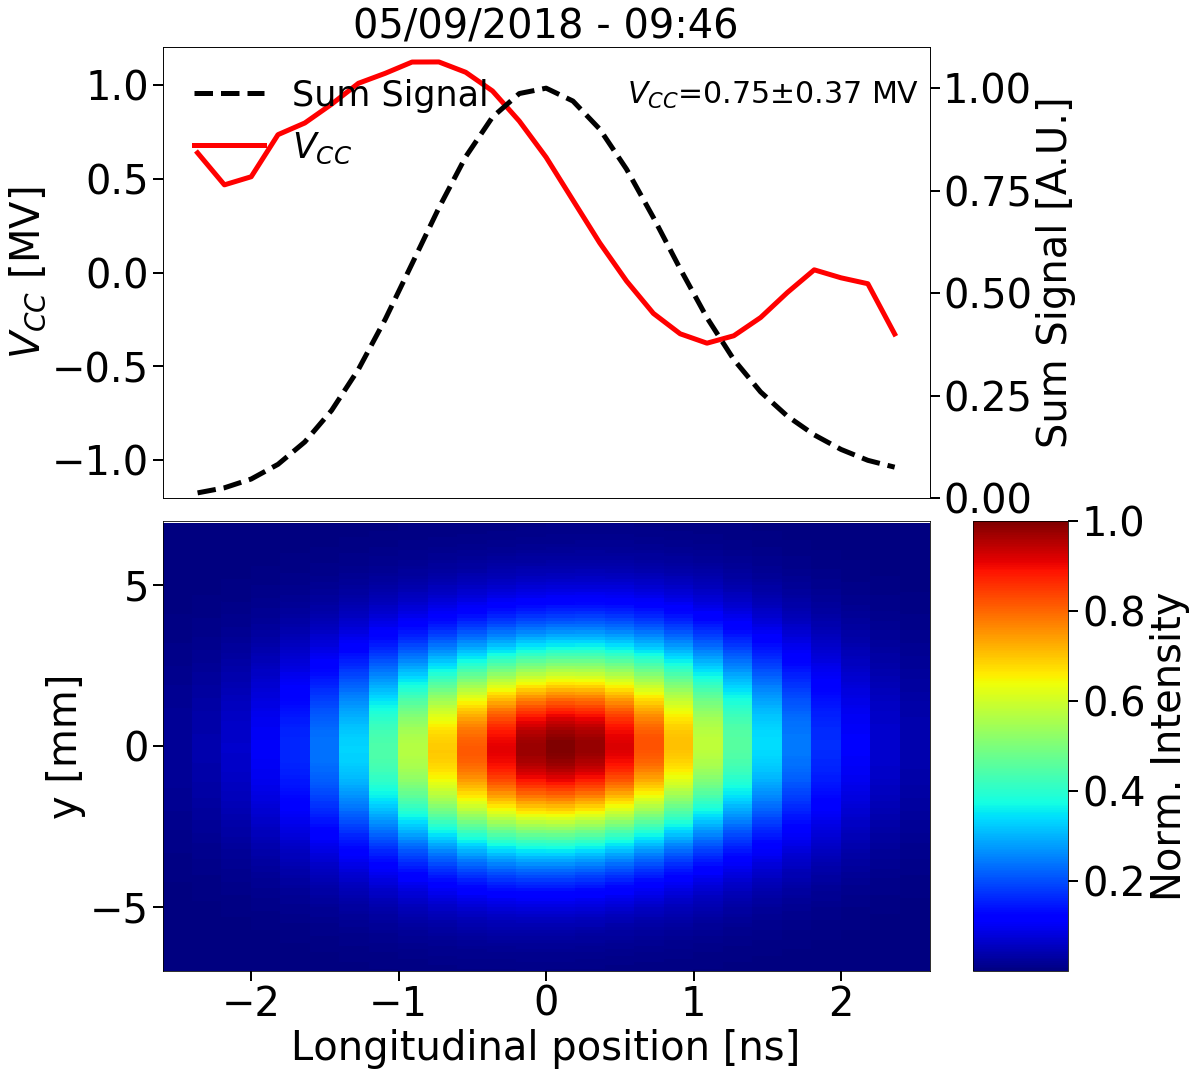
\includegraphics[width=1\textwidth]{images/Ch5/HT_crabVoltage__20180905_094640_crabbing_only.png}
        %\caption{$y=\sin(2 \pi f t),\ f=50$ Hz}
        %\label{fig:signal_and_DFT_example_a}
    \end{subfigure}
    \hfill
    \begin{subfigure}[t]{0.45\textwidth}
        \centering
        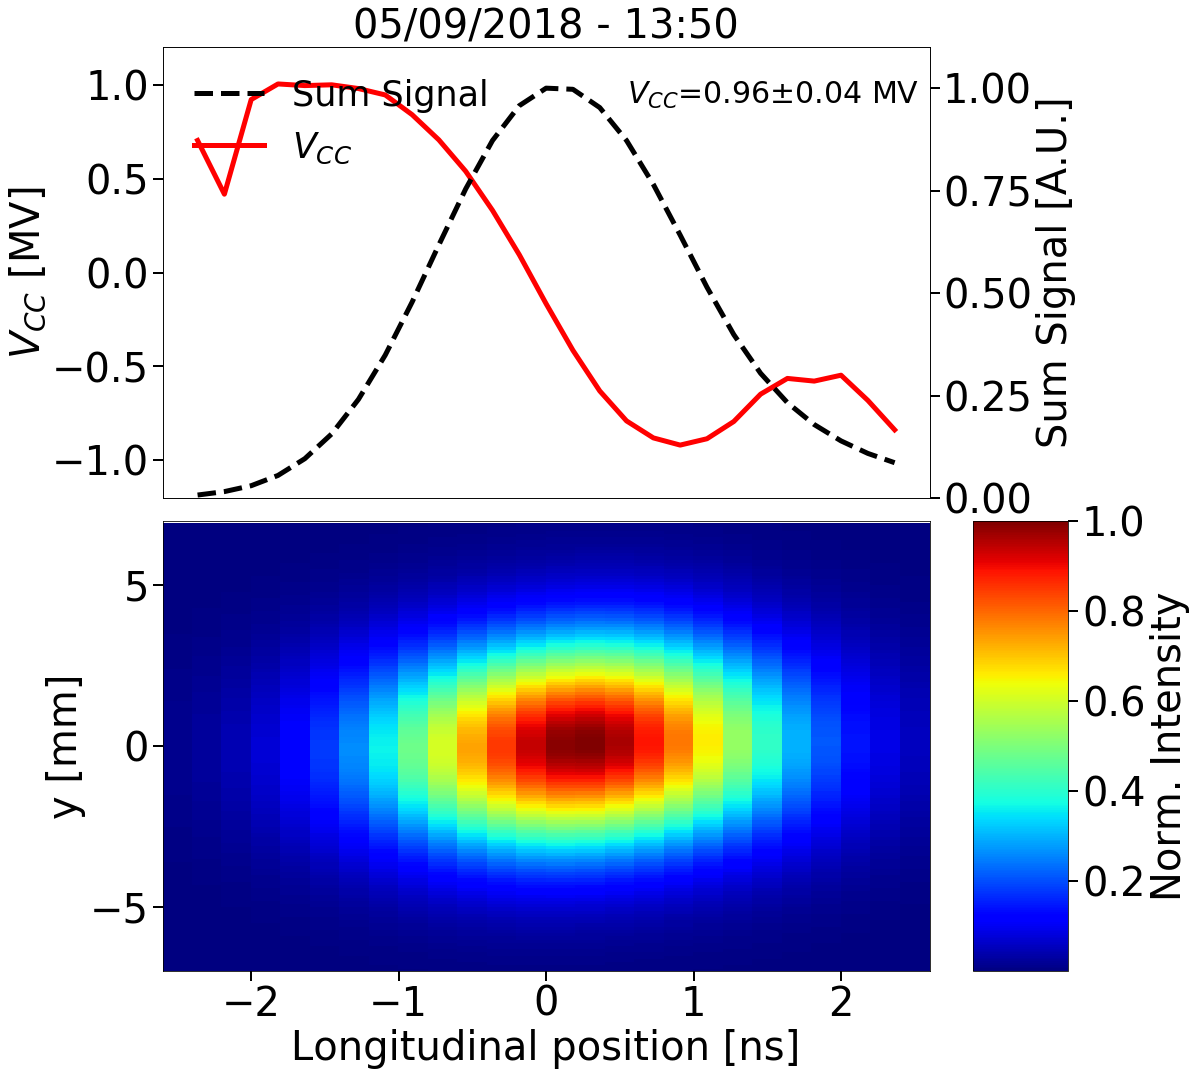
\includegraphics[width=1\textwidth]{images/Ch5/HT_crabVoltage__20180905_135033_crabbing_only.png}
        %\caption{Discrete Fourier transform}
        %\label{fig:signal_and_DFT_example_b}
    \end{subfigure}
    \hfill
     \caption{Measured CC voltage before (left) and during (right) the emittance growth studies, together with the schematic represantation of the crabbing (bottom) as introduced in Fig.~\ref{fig:crabbing_reconstruction_HT_monitor}. The voltage callibration was done from the HT monitor acquisitions as discussed in Section~\ref{subsec:HT_post_process_CC}. }
     \label{fig:VCC_MD5_2018} 
\end{figure}

% Observation: 1. Signals assymetric. Enhanced due to higher energy 2. the crabbing is less visible in the density plots due to higher energy. 3. We assume that the CC settings didnt change throught the coast. 4. The experts appear confident that the votlage was 1 MV.
\begin{sloppypar} % to fix \hbox too wide
The $\CC$ voltage is estimated, from the peak to peak amplitude, at 0.76\,MV and 0.97\,MV from the first and second acquisition respectively. For the direct comparison of the measured growth rates with measuremnts and simulations (section.. ) and Ch... the average of the two values is used, $\VCC$ = 0.865\,MV. \textcolor{red}{The unceratinties on the Vcc to be discussed.} This consideration is based on the assumption that the $\CC$ settings remained unchanged during the experiment.
\end{sloppypar} 

\section{Injected RF noise}\label{sec:noise_meas2018}
\begin{sloppypar} % to fix \hbox too wide
 The injected noise was a mixture of amplitude and phase noise up to 10\,kHz, overlapping and primarily exciting the first betatron sideband at $\sim 8$\,kHz. The phase noise was always dominant. Figure~\ref{fig:example_PN_and_AN} dsiplays two example measurements of phase (left) and amplitude (right) noise acquired during the experiment with a sepctrum analyzer E5052B~\cite{E5052B_insight}. 
\end{sloppypar} 

 % Loaction for creating the figure: /eos/user/n/natriant/2018/CC_MD_2018_summary/measured_psd
 \begin{figure}[!ht]
    \centering
    \begin{subfigure}[t]{0.45\textwidth}
        \centering
        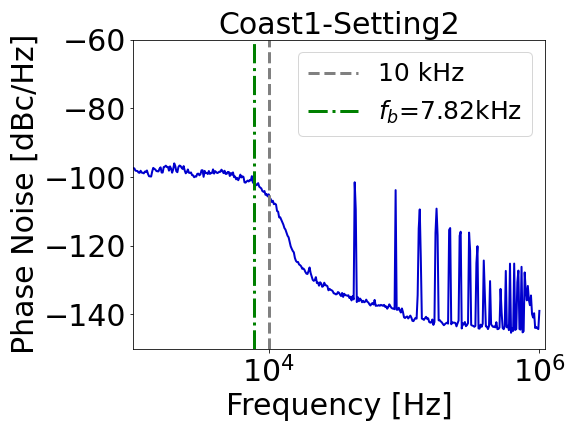
\includegraphics[width=1\textwidth]{images/Ch5/Measured_spectrum_MD5_Coast1-Setting2-PN.csv_no_psd.png}
        %\caption{$y=\sin(2 \pi f t),\ f=50$ Hz}
        %\label{fig:add_label_here}
    \end{subfigure}
    \hfill
    \begin{subfigure}[t]{0.45\textwidth}
        \centering
        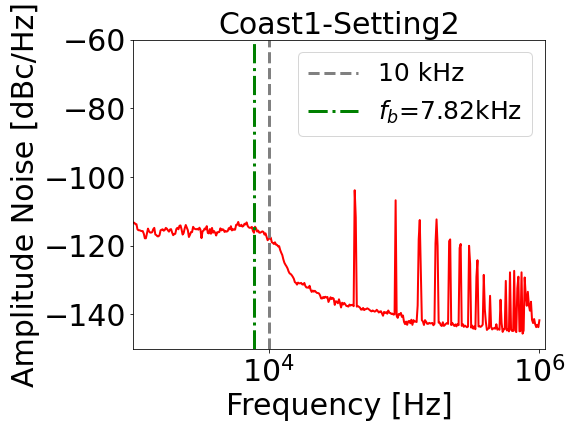
\includegraphics[width=1\textwidth]{images/Ch5/Measured_spectrum_MD5_Coast1-Setting2-AN.csv_no_psd.png}
        %\caption{Discrete Fourier transform}
        %\label{fig:add_label_here}
    \end{subfigure}
    \hfill
     \caption{Example phase (left) and amplitude (right) noise spectra measured with a spectrum analyzer E5052B during the emittance growth studies with CCs in SPS. The noise spread-out up to 10\,kHz (grey dashed line) exciting the first betatron sideband at $\sim$8\,kHz (green dashed line). The spikes at high frequencies correspond to the harmonics of the revolution frequency and are a result of the bunch crossing.} % bunch passage
     \label{fig:example_PN_and_AN}
\end{figure}



\textcolor{red}{The following needs to be refined. I struggled to write it}.
\begin{sloppypar} 
Emittance growth measurements were performed for seven different noise levels, listed in Table~\ref{tab:noise_settings_2018}. The following two points should be highlighted regarding its listings. 
\begin{itemize}
    \item As already discussed in Chapter~\ref{Ch:CC_noise_theory} the noise induced emittance growth depends on the noise power at the beteatron and synchrobetatron sidebands for the phase and amplitude noise respectively (see Eq.~\ref{eq:dey_pn} and Eq.~\ref{eq:dey_an}). Therefore, the noise power values of interest for this thesis are the ones at the first betatron $f_b = 0.18 \times \frev$ = 7.82\,kHz and at the synchrobetatron sidebands at $f_b \pm \Qs \times \frev  = f_b \pm  \sim 220$\,kHz. In the following, it is assumed for simplicity that the noise power at the sidebands mentioned above is the same. Here this assumption is acceptable since the noise power in the measurements is basically constant for all frequencies up to 10\,KHz. 
    \item It is clear from Fig.~\ref{fig:example_PN_and_AN} that the measurements are noisy. In particular random changes in amplitude are observed from point to point within the signal. The values listed in Table~\ref{tab:noise_settings_2018} correspond to the averaged noise values over a frequency range of $\pm$ 500\,Hz around the betatron frequency. The unceratinties show the spread of the values and are defined 
\end{itemize}

\end{sloppypar} 

\begin{table}[!hbt]
	\centering
   \caption{Phase and amplitude noise levels injected in the CC RF system for the emittance growth studies in 2018.}
	\begin{tabu} to \textwidth { X[c,m] X[c,m] X[c,m] X[c,m] }
		&&& \\[-6mm]
		\toprule \toprule
		\multicolumn{2}{l}{} &
		\multicolumn{2}{c}{$\mathbf{10\,\boldsymbol{\log}_{10} \mathcal{L}(f)}$ \textbf{[dBc/Hz]}} \\
		\bottomrule
      \multicolumn{2}{l}{} & 	\multicolumn{1}{c}{\textbf{Phase noise}} & \multicolumn{1}{c}{\textbf{Amplitude noise}} \\
      \midrule
      \multicolumn{2}{l}{Coast1-Setting1}  & \multicolumn{1}{c}{-122.6 $\pm 0.6$} & \multicolumn{1}{c}{-128.1 $\pm$ 0.6} \\
      
      \multicolumn{2}{l}{Coast1-Setting2}  & \multicolumn{1}{c}{-101.4 $\pm$ 0.8} & \multicolumn{1}{c}{-115.2 $\pm$ 0.6} \\

      \multicolumn{2}{l}{Coast2-Setting1}  & \multicolumn{1}{c}{-115.1 $\pm$ 0.8} & \multicolumn{1}{c}{-124.1 $\pm$ 0.5} \\

      \multicolumn{2}{l}{Coast2-Setting2}  & \multicolumn{1}{c}{-111.4 $\pm$ 0.6} & \multicolumn{1}{c}{-115.7 $\pm$ 0.4} \\ 

      \multicolumn{2}{l}{Coast3-Setting1}  & \multicolumn{1}{c}{-110.9 $\pm$ 0.9} & \multicolumn{1}{c}{-116.9 $\pm$ 0.4} \\

      \multicolumn{2}{l}{Coast3-Setting2} & \multicolumn{1}{c}{-106.4 $\pm$ 0.3} & \multicolumn{1}{c}{-112.9 $\pm$ 0.6} \\

      \multicolumn{2}{l}{Coast3-Setting3} & \multicolumn{1}{c}{-101.4 $\pm$ 0.7}  & \multicolumn{1}{c}{-106.9 $\pm$ 0.5} \\
      \arrayrulecolor{black}\bottomrule
 
	\end{tabu}
   \label{tab:noise_settings_2018}
\end{table}



\begin{sloppypar} % to fix \hbox too wide
This spectrum analyzer provides a single sideband measurement (SSB), which is expressed as $10\log_{10}\mathcal{L}(f)$\,[dBc/Hz]. Its relation with the power spectral densities (PSDs) introduced in Eq.~\eqref{eq:dey_an} and Eq.~\eqref{eq:dey_pn} are given by $S_\Delta = 2\mathcal{L}(f)$~\cite{IEEE:4797525}, with $S_{\Delta A}$ in 1/Hz and $S_{\Delta\phi}$ in rad$^2$/Hz. A detailed discussion on the noise power measurements and their relation to the mathimatical defintion of the PSD is given in Chapter [tba].

As already mentioned above, the injected noise was a combination of both phase and amplitude noise. Therefore, in order to make a meaningful comparison between the different noise levels the concept of effective phase noise is introduced. This is the phase noise level that would lead to
the same emittance growth as that from both phase and
amplitude noise. The noise levels mentioned in this chapter correspond to the calculated effective phase noise.
% should I slightly change this paragraph? Too much copy paste from IPAC or it's ok?
\end{sloppypar} 



\section{Emittance growth measurements}\label{sec:EmitGrowth_measurements}

An overview of the emittance growth measurments is shown in Fig ... for both horizontal (top) and vertical (bottom) plane. The three "coasts" are distinguishable with the black dashed vertical lines. For each "coast" a nea beam was injected with the same targeted initial conditions. The different levels of injected noise are displayed in the plot (bottom) while the moments at which the noise level changed are shown with the grey dashed vertical lines. These noise levels correspond to the average of the effective phase noise over the four bunches



Seven different noise levels were studied

The measurements for characterizing the $\CC$ noise induced emittance growth lasted ~ 7 hours. The emittance evolution was recordered for seven different noise levels. 

Seven different noise levels were i


As already mentioned the measurements for studying the emittance growth started aroung
The emittance evolution for the seven dif

The three different "coasts" are easily distinguishable with the dashed black lines while the evolution of the beam during the different noise settings is shown with the grey vertical lines. The 4 colors correspons to the four different bunches. 

What shold be observed is the following: ...

% Figures for emit growth evolution MD 2018: SWAN_projects/CC_MDs_2018/myAnalysis_2020/for_thesis/average_MD5_overview_5Sep2018_emitBU_PlotOverview_Vertical_OpenRatesFromPickle_for_thesis.ipynb


- For the AN we are interested in fb+-qs. however we consider its flat and we keep the value of fb. Nevetherless the impact from the AN should be very small.

MD emittance growth overview. 
    - average from IN and OUT. As mentioned in CH4. vs time and vs noise level for all bunches. Not yet comparison with the theory. Probably you need to re-run this to make correctly the error propagation. 
    - 1 noise point was excluded
 


\section{Bunch length measurements}\label{sec:bunch_length_measurements_2018}
    - bunch length and longitudinal profiles and relative position from the wall current monitor.  unstable bunches.
    - bunch 2-3-4 longutidinally unstable.
 
\section{Intensity measurements}\label{sec:intensity_measurements_2018}
No losses. Maybe not seperate chapter?
I should also mention in Ch4 how the emittance is measured from the ABWLM.

\section{Comparison of measured emittance growth with the theory}\label{sec:meas_2018_vs_theory}

Comparison of bunch 1 with theory. Discrepancy of a factor 4.


 \section{Conclusions and outlook}\label{sec:MD2018_summary}
